\documentclass[10pt,a4paper]{article}
\usepackage[a4paper]{geometry}

\usepackage{polski}
\usepackage{xltxtra}
\usepackage{relsize}
\usepackage{fancyvrb}
\usepackage[pdfborder={0 0 0}]{hyperref}
\usepackage{booktabs}
\usepackage{graphicx}

\defaultfontfeatures{Mapping=tex-text}
\setromanfont{Charis SIL}
\setmonofont[Scale=MatchLowercase]{Menlo}
\linespread{1.25}

\DefineVerbatimEnvironment%
  {SmallVerbatim}%
  {Verbatim}{fontsize=\relsize{-0.5},numbers=left,numbersep=-10pt,frame=lines,tabsize=4}

\newcommand{\prog}[1]{\texttt{#1}}

\begin{document}

%%fakesection{Tytuł}
\title{ 
  Interpolacja funkcjami sklejanymi\\
  {\normalsize Specyfikacja funkcjonalna projektu nr 2}\\\vspace{-12pt}
  {\normalsize z przedmiotu \emph{Języki i metody programowania 2}}
}
\author{
  Tomasz Cudziło\\
  {\small EE PW, 211552}
}
\date{\today}
\maketitle

\section*{Zadanie}
\label{sec:zadanie}

Napisać program, z~graficznym interfejsem użytkownika, wyznaczający
współczynniki funkcji sklejanych trzeciego stopnia aproksymujących zadany ciąg
danych pomiarowych.

\vspace{24pt}

\section{Opis}
\label{sec:opis}

Poprzez GUI aplikacja pozwala na:
\begin{itemize}
  \item wczytanie z~pliku lub ręczne wprowadzenie danych wejściowych
    i~wyświetlenie wyliczonych funkcji na wykresie,
  \item wczytanie z~pliku wyliczonych funkcji sklejanych i~wyświetlenie ich na
    wykresie,
  \item edycję wczytanych punktów, zapis wprowadzonych zmian oraz eksport
    wyliczonych wielomianów,
  \item zoom i~scroll wykresu,
  \item eksport wykresu do pliku.
\end{itemize}

Program jest front-endem do programu \prog{splines} z projektu pierwszego i~nie
rozszerza jego funkcjonalności w~znaczący sposób. Rysowanie i~eksport wykresów
do plików jest wykonywany za pomocą \prog{gnuplot}.

\section{Obsługa}
\label{sec:obsluga}

Aplikacja korzysta z~jednego okna głównego oraz kilku pomocniczych okien
dialogowych.

\subsection{Okno główne}

Okno główne (rysunek nr~\ref{fig:okno-glowne}) zawiera z~lewej strony
tabelę z~punktami. Jej zawartość można edytować. W~prawej, górnej ćwiartce
znajduje się pole na wykres. Pod wykresem jest tabela z~wyznaczonymi
wielomianami i~ich przedziałami.

Wykres można przybliżać korzystając z~ze skrótów klawiaturowych opisanych
w~tabeli \ref{tab:skroty} na stronie \pageref{tab:skroty}. Przesuwanie jest
dostępne wykorzystując paski na obrzeżach lub scroll myszki.

Wielomiany i~wykres są aktualizowane automatycznie przy każdej zmianie punktów
w~tabeli.

\begin{figure}[hb]
  \centering
  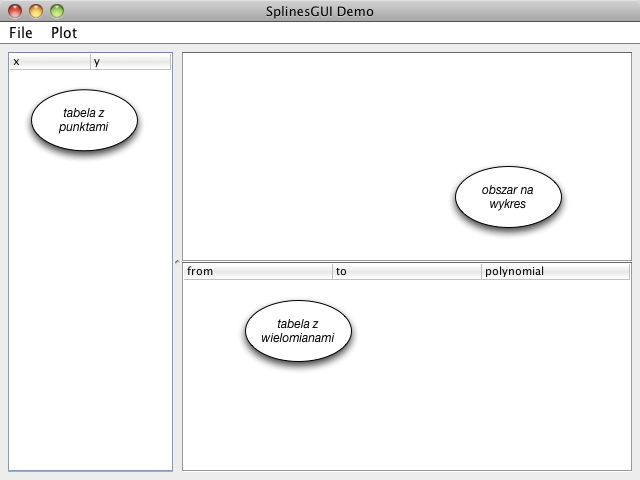
\includegraphics[width=\textwidth]{images/okno-glowne}
  \caption{Okno główne aplikacji.}
  \label{fig:okno-glowne}
\end{figure}

\subsection{Okna pomocnicze}

\subsubsection{Okno eksportu wykresu}

Aplikacja pozwala na eksport wykresu do pliku. Po wyborze akcji z~menu okna
głównego, pojawia się modalne okno dialogowe (rysunek
\ref{fig:eksport-wykresu}), pytające o~docelowe rozmiary i~format pliku.
Następnie pojawia się standardowe okno dialogowe do wskazania miejsca zapisu.

\begin{figure}[h]
  \centering
  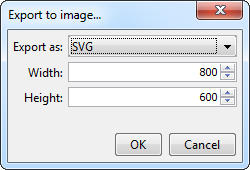
\includegraphics[width=0.374\textwidth]{images/eksport-wykresu}
  \caption{Okno dialogowe z~wartościami do eksportu wykresu.}
  \label{fig:eksport-wykresu}
\end{figure}

\subsubsection{Okno wyboru pliku}

W~pozostałych przypadkach wykorzystywane jest standardowe okno wyboru pliku.

\begin{table}[p]
  \centering
  \begin{tabular}{l c}
    \toprule
    \multicolumn{1}{c}{\bf Akcja} & {\bf Skrót} \\
    \midrule
    otwórz plik              &  \verb|^O|  \\
    zamknij aplikację        &  \verb|^Q|  \\
    zapisz punkty            &  \verb|^S|  \\
    zapisz wielomiany        &  \verb|^D|  \\
    eksport wykresu          &  \verb|^E|  \\
    eksport do {\tt gnuplot} &  \verb|^G|  \\
    \midrule
    zoom in                  &  \verb|^+|  \\
    zoom out                 &  \verb|^-|  \\
    zoom 100\%               &  \verb|^0|  \\
    obszar wykresu           &  \verb|mysz|  \\
    \bottomrule
  \end{tabular}
  \caption{Skróty klawiaturowe aplikacji.}
  \label{tab:skroty}
\end{table}

\section{Pliki}
\label{sec:pliki}

\section{Wymagania}
\label{sec:wymagania}

Warunki potrzebne do uruchomienia aplikacji:
\begin{itemize}
  \item dostępna \prog{JVM},
  \item dostępny pakiet \prog{gnuplot} w wersji \prog{>= 4.4},
  \item binarka projektu nr~1 widoczna z~\prog{PATH}.
\end{itemize}

\end{document}
